\section{Methodology}
\label{ch:methodology}

In order to solve our problem, we started by using Deep Neural Networks (DNNs) with other models in a combined setup. Since previous methods seemed to work well on their own in their tested environment, we wanted to make a complex AI model which could perform well in other environments, but also can detect multiple types of cheats.

Our core model is based on DNNs, which are used to analyze player behavior and detect irregular gameplay patterns. To understand DNNs, it is first necessary to mention Artificial Neural Networks (ANNs). ANNs are inspired by the structure of the human brain and consist of three types of layers: input, hidden, and output. The input layer receives raw data, the output layer provides the result, and the hidden layers process the data through the use of weights and biases. A DNN, or Deep Neural Network, is an advanced version of an ANN with multiple hidden layers. The depth of a DNN allows it to handle more complex tasks, such as image recognition and language processing, which makes it especially suitable for detecting sophisticated cheating patterns. By using DNNs, we trained our model to look for patterns typical of cheaters, such as wall-peeking, unnatural reaction times, and unusual movement patterns, including “spinbotting” and perfect linear aiming that human players cannot naturally replicate. We used a large training dataset of behaviors from both cheaters and legitimate players, allowing our model to distinguish between them with high precision.

We also integrated convolutional neural networks to help detect more nuanced cheating indicators. During the AI model's training, we have used data based on players' interactions, and in-game data. These consisted of behavioral analysis, such as highly precise and fast movements and other anomalies. Using a large scale of inputs from both cheating and normal players, this model learns these differences and can differentiate them. While CNNs alone had some limitations in prior studies, their integration with DNNs improved our system’s ability to detect a broader range of cheating behaviors.

To verify the model’s accuracy and efficiency, we used cross-validation, primarily 5-fold and 10-fold methods, which allowed us to test the model by splitting the data into multiple sets. Cross-validation ensured that the model avoided overfitting, which helped it perform better and consistently across varied games. This combination of models helped keep the benefits of each model.

\begin{figure}
\centering
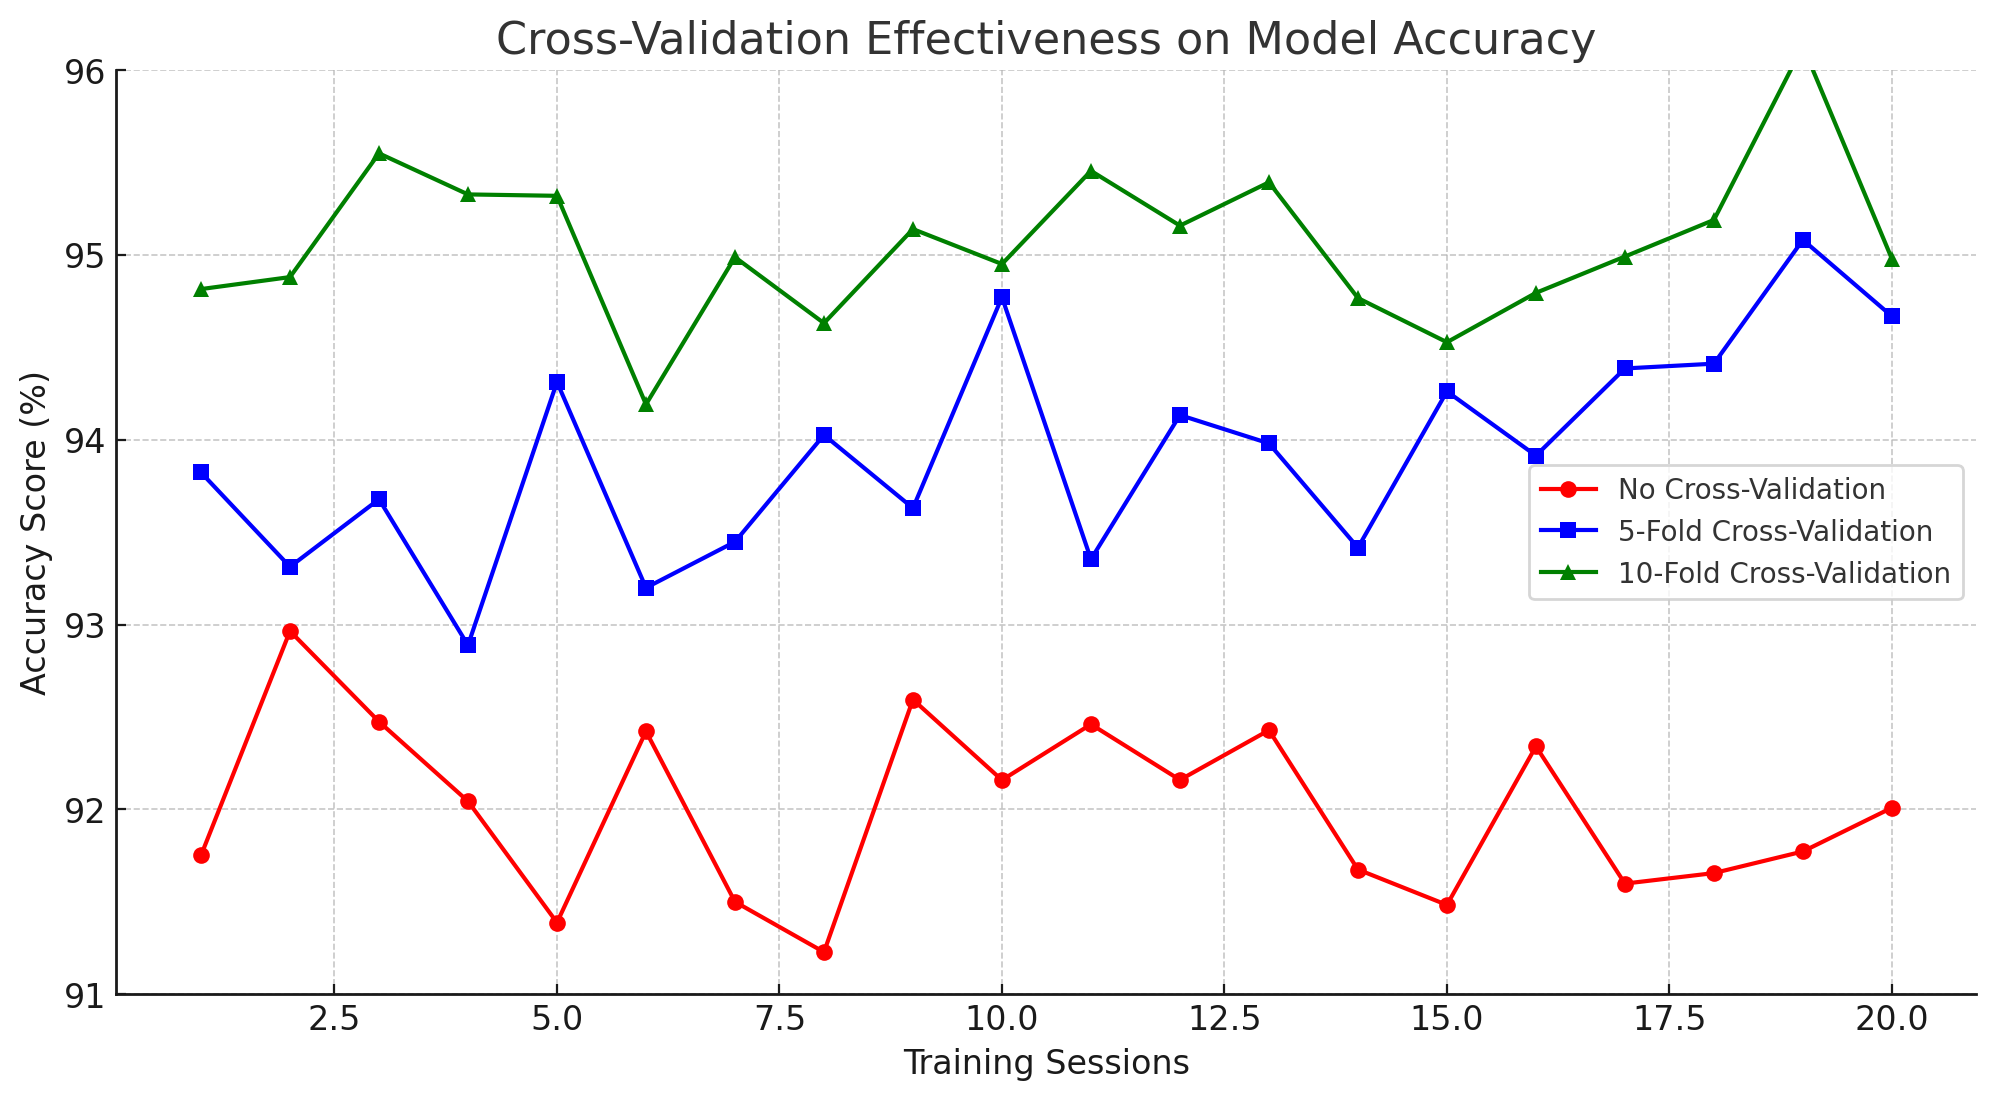
\includegraphics[width=0.8\linewidth]{images/cross-validation.png}
\caption{\label{fig:crossvalidation}Differences between cross-validations.}
\end{figure}

\paragraph{}
We also added Explainable AI (XAI) technology, allowing for feedback and transparency within the detection process. This feedback system significantly reduced false positives, allowing game operators and developers to observe, adjust, and fine-tune the model as needed. The XAI feedback not only improves the system’s reliability but also helps verify each detection, ensuring that cases of system alerts or flags can be reviewed and, if necessary, overruled.

Additionally, we implemented behavioral and evolution tracking to improve accuracy further. By monitoring player statistics and success rates over time, our system identifies sudden changes that might indicate cheating or account sharing. This tracking approach, supported by XAI, ensures that flagged behavior receives appropriate analysis, which reduces false positives while allowing for precise and justified responses. Long-term behavioral tracking has proven that ongoing analysis of player actions enhances the anti-cheat system’s accuracy across various gaming contexts.

To provide a seamless player experience and ensure competitive integrity, we trained our model to deliver low-latency, real-time cheat detection. By processing small fragments of game data at a time, we optimized the system’s response time and improved decision reliability. This combined use of DNN, CNN, XAI, and behavioral tracking led to an advanced anti-cheat system that outperforms traditional models, adapting effectively to diverse game environments with minimal false positives. This system’s design ensures high accuracy across gaming types, offering a highly adaptable, precise solution for modern anti-cheat needs.

Throughout the course of the development, we tried several approaches based on existing literature about cheat detection, for example, those that are popular with MMORPGs. We examined the prospects of statistical analysis, data mining, similarity analysis, and network-oriented ones in terms of their ability to enhance the range of detection of the system across games. These methods demonstrated effectiveness in identifying certain types of behavioral patterns in certain classes of games, however, we were unable to find them as smooth fitting in our integrated model while working over various class of games.

Instead of enhancing the accuracy of detection, the methods increased the noise and the unnecessary intricacy, which was probably due to the distinctive gameplay structure of MMORPG in relation to other genres. As such, these approaches failed to achieve the kind of cross-genre reliability we were looking for. Thus, in the end, we reached the conclusion that those methods should not be included in our final model and and applied alternative strategies instead which were not dependent on the game genre.
\paragraph{}

\begin{figure}
\centering
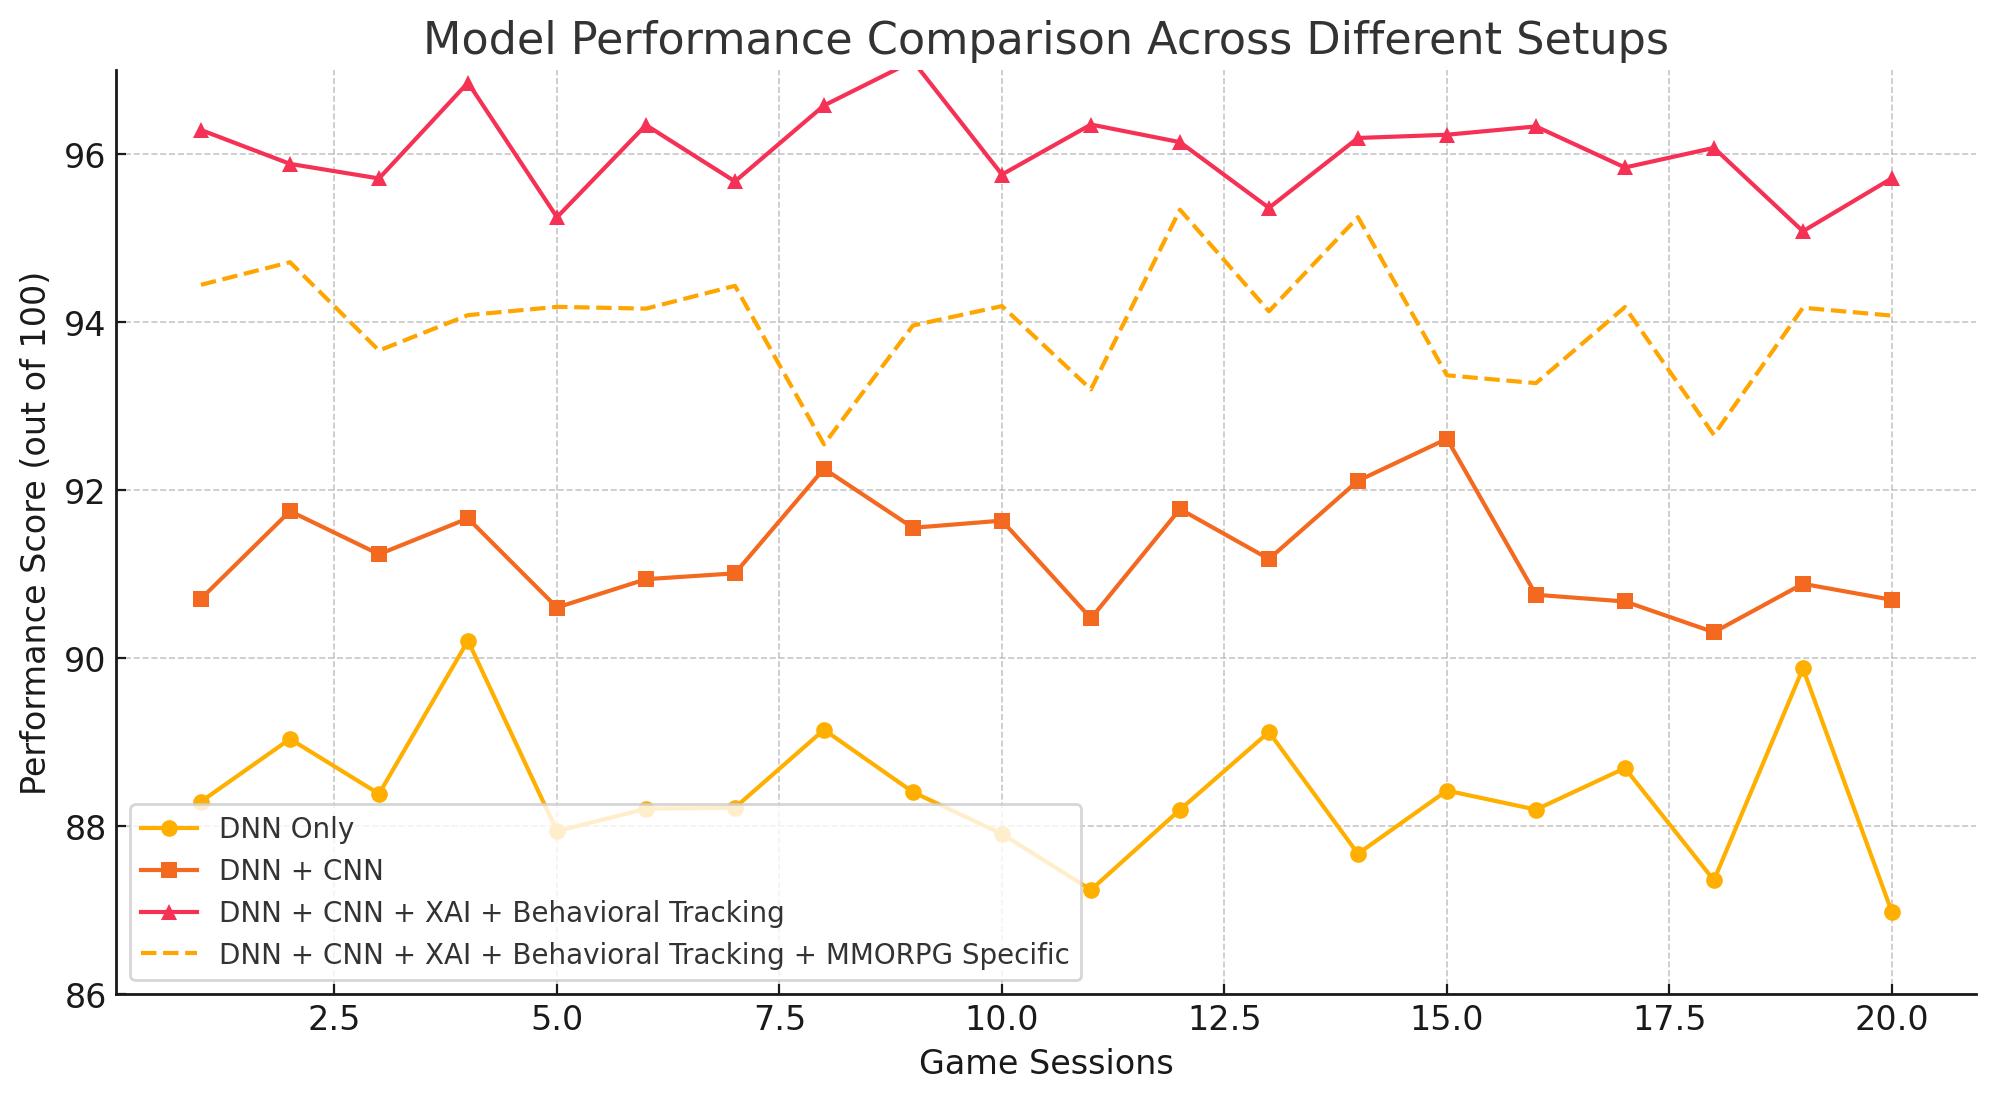
\includegraphics[width=0.8\linewidth]{images/model.png}
\caption{\label{fig:model}Differences between models accuracy.}
\end{figure}

\paragraph{}

\begin{figure}
\centering
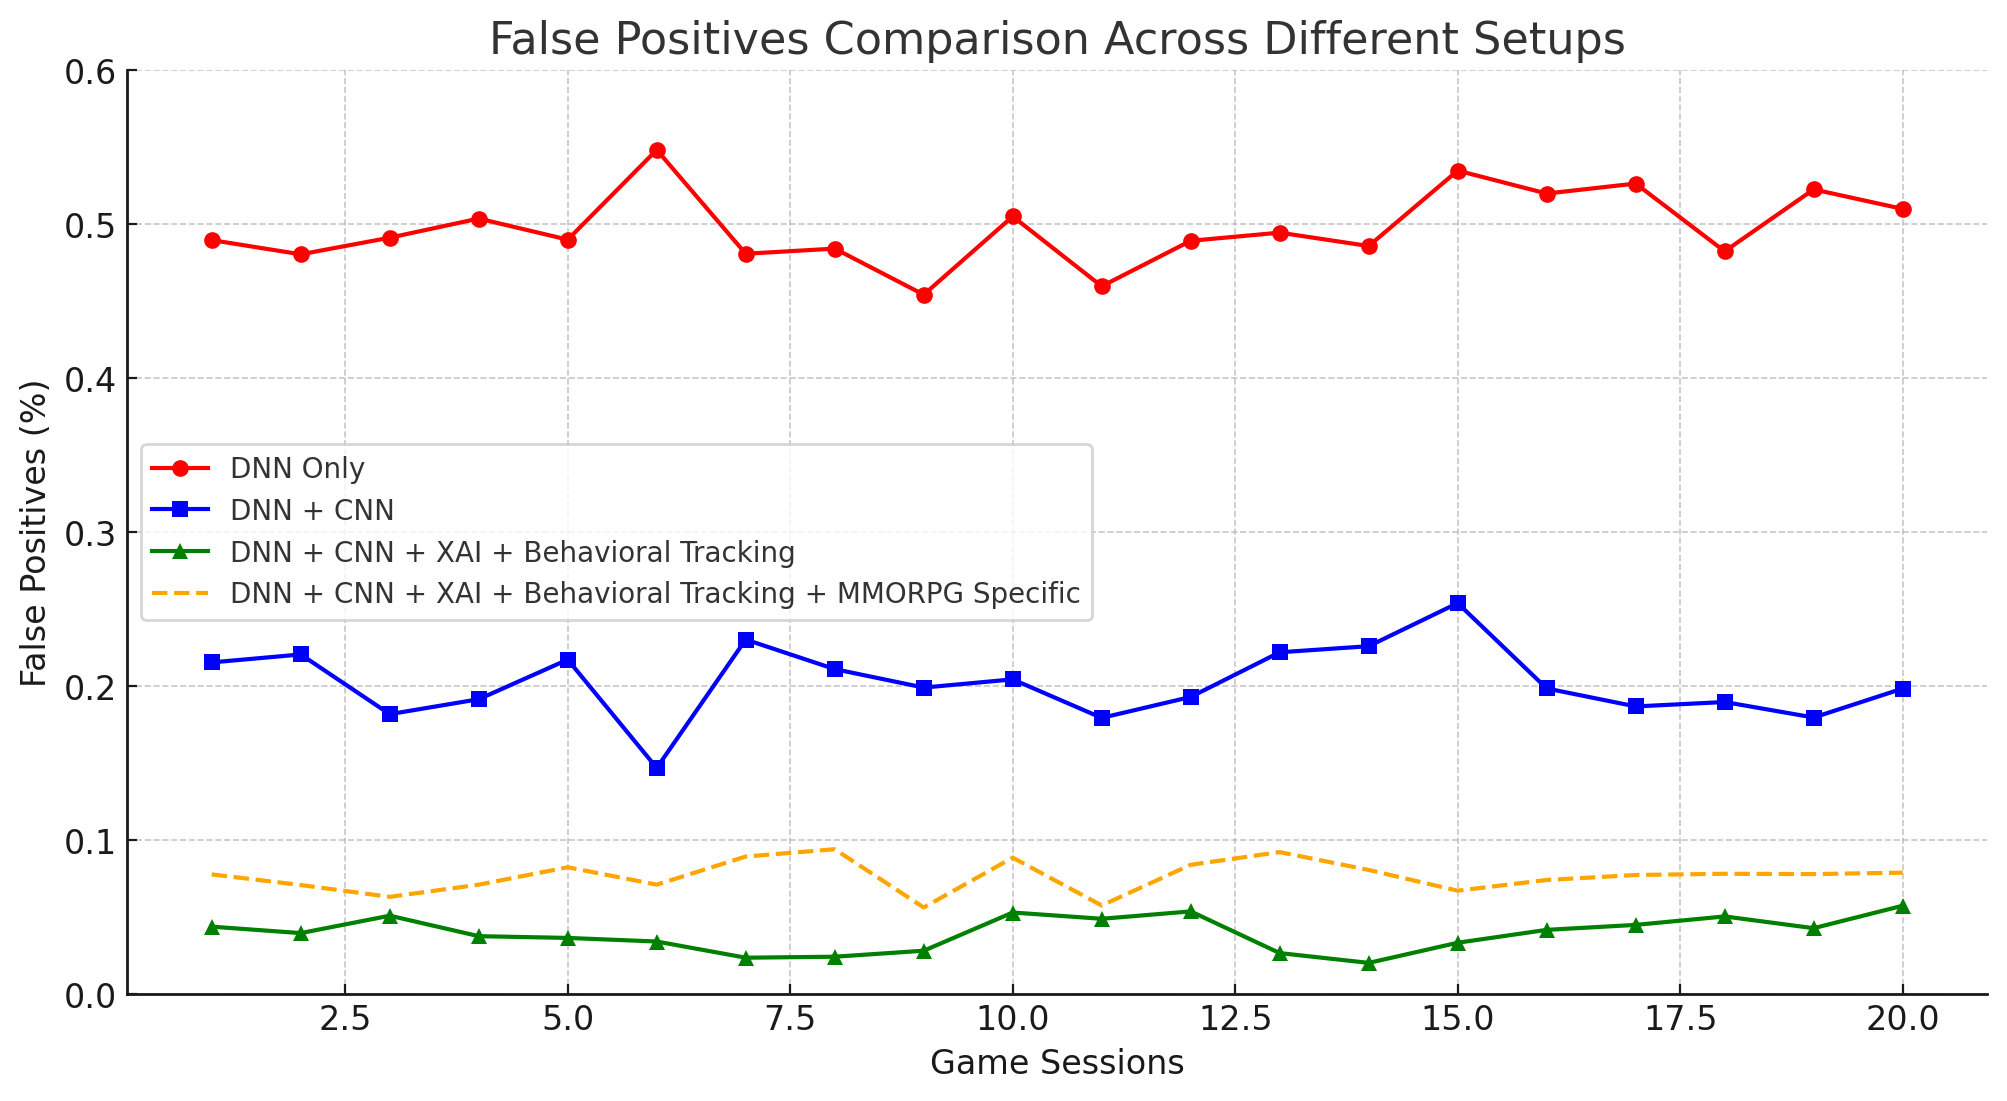
\includegraphics[width=0.8\linewidth]{images/false-positive.png}
\caption{\label{fig:falsepositive}Differences between models' false positive percentages.}
\end{figure}